\let\negmedspace\undefined
\let\negthickspace\undefined
\documentclass[journal]{IEEEtran}
\usepackage[a5paper, margin=10mm, onecolumn]{geometry}
%\usepackage{lmodern} % Ensure lmodern is loaded for pdflatex
\usepackage{tfrupee} % Include tfrupee package

\setlength{\headheight}{1cm} % Set the height of the header box
\setlength{\headsep}{0mm}     % Set the distance between the header box and the top of the text

\usepackage{gvv-book}
\usepackage{gvv}
\usepackage{cite}
\usepackage{amsmath,amssymb,amsfonts,amsthm}
\usepackage{algorithmic}
\usepackage{graphicx}
\usepackage{textcomp}
\usepackage{xcolor}
\usepackage{txfonts}
\usepackage{listings}
\usepackage{enumitem}
\usepackage{mathtools}
\usepackage{gensymb}
\usepackage{comment}
\usepackage[breaklinks=true]{hyperref}
\usepackage{tkz-euclide} 
\usepackage{listings}
% \usepackage{gvv}                                        
\def\inputGnumericTable{}                                 
\usepackage[latin1]{inputenc}                                
\usepackage{color}                                            
\usepackage{array}                                            
\usepackage{longtable}                                       
\usepackage{calc}                                             
\usepackage{multirow}                                         
\usepackage{hhline}                                           
\usepackage{ifthen}                                           
\usepackage{lscape}
\usepackage{tikz}
\usepackage{textcomp}
\usetikzlibrary{circuits.ee.IEC, positioning}
\begin{document}

\bibliographystyle{IEEEtran}
\vspace{3cm}

\title{10.3.4.2.5}
\author{Manognya Kundarapu - EE24BTECH11037
}
% \maketitle
% \newpage
% \bigskip
{\let\newpage\relax\maketitle}

\renewcommand{\thefigure}{\theenumi}
\renewcommand{\thetable}{\theenumi}
\setlength{\intextsep}{10pt} % Space between text and floats


\numberwithin{equation}{enumi}
\numberwithin{figure}{enumi}
\renewcommand{\thetable}{\theenumi}
\textbf{Question:} A lending library has a fixed charge for the first three days and an additional charge for each day thereafter. Saritha paid  Rs. 27 for a book kept for seven days, while Susy
paid  Rs. 21 for the book she kept for five days. Find the fixed charge and the charge
for each extra day.
\begin{enumerate}
    \item \textbf{Theoretical Solution:}\\ 
    Let the fixed charge be Rs. $x$ and the additional charge per day be Rs. $y$ \\
    \begin{align}
        \implies x+4y=27\\
        x+2y=21\\
        \text{From 1.1, }x=\brak{27-4y}\\
        \text{Substituting $x$ in 1.2, we get  }\brak{27-4y+2y}=21\\
        \implies y=3\\
        x=15\\
        \therefore \text{The fixed charge is Rs. 15 and extra charge per day is Rs. 3}
    \end{align}
    \item \textbf{LU Decomposition using Doolittle's algorithm}\\
    The system of linear equations: $x+4y=27$ and $x+2y=21$ can be written in matrix form as;\\
    \begin{center}
        $A\Vec{x} = \Vec{b}$, where\\
        \vspace{0.5cm}
        $A = \begin{bmatrix} 
1 & 4 \\ 
1 & 2 
\end{bmatrix}, \quad
\Vec{x} =
\begin{bmatrix} 
x \\ 
y 
\end{bmatrix}, 
\quad
 \Vec{b} =
\begin{bmatrix} 
27 \\ 
21 
\end{bmatrix}
$
    \end{center}
    Doolittle's algorithm decomposes $A$ into a lower triangular matrix $L$ and an upper triangular matrix $U$ such that:
\[
A = LU
\]
where:
\[
L =
\begin{bmatrix} 
1 & 0 \\ 
l_{21} & 1
\end{bmatrix},
\quad
U =
\begin{bmatrix} 
u_{11} & u_{12} \\ 
0 & u_{22}
\end{bmatrix}
\]
The elements of \( L \) and \( U \) are computed using:
\begin{align}
    U[i][j] &= A[i][j] - \sum_{k=0}^{i-1} L[i][k] U[k][j] \\
    L[i][j] &= \frac{A[i][j] - \sum_{k=0}^{j-1} L[i][k] U[k][j]}{U[j][j]}
\end{align}
with the constraint \( L[i][i] = 1 \).\\
Thus, we obtain\\ \[
L =
\begin{bmatrix} 
1 & 0 \\ 
1 & 1
\end{bmatrix},
\quad
U =
\begin{bmatrix} 
1 & 4 \\ 
0 & -2
\end{bmatrix}
\]\\
\textbf{Solving for \( \Vec{x} \) using Forward and Backward Substitution}\\
With \( A = LU \), we solve:
\[
L\Vec{y} = \Vec{b}
\]
\begin{center}
    $\begin{bmatrix} 
1 & 0 \\ 
l_{21} & 1
\end{bmatrix}
\begin{bmatrix} 
y_1 \\ 
y_2
\end{bmatrix} = \begin{bmatrix} 
27 \\ 
21
\end{bmatrix}$
\end{center} 
Solving step-by-step:\\
\begin{center}
    $\Vec{y}=\begin{bmatrix} 
27 \\ 
-6
\end{bmatrix}$
\end{center}
\textbf{Backward Substitution}\\
Expanding \( U\Vec{x}= \Vec{y}\):
\[
\begin{bmatrix} 
1 & 4 \\ 
0 & -2
\end{bmatrix}
\begin{bmatrix} 
x \\ 
y
\end{bmatrix}
=
\begin{bmatrix} 
27 \\ 
-6
\end{bmatrix}
\]\\
Thus we obtain; \\
\begin{center}
    $\Vec{x}=\begin{bmatrix} 
15 \\ 
3
\end{bmatrix}$
\end{center}
\end{enumerate}
\begin{figure}[htbp]
  \centering
  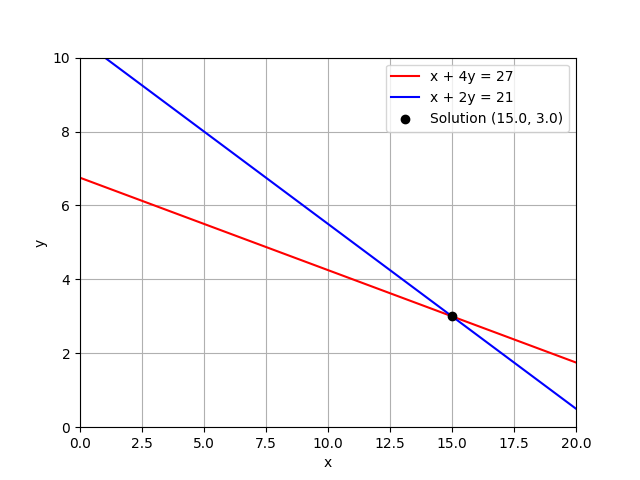
\includegraphics[width=\columnwidth]{figs/curve.png}
\end{figure}
\end{document}
